\documentclass[tikz,fontsize=8pt]{standalone}
\usepackage{fourier}
\usetikzlibrary{arrows.meta}
\usetikzlibrary{calc}
\tikzset{>=latex}
\definecolor{bookblue}{RGB}{0,173,239}
\definecolor{bookpink}{RGB}{236,0,140}
\definecolor{bookgreen}{RGB}{50,200,0}
\definecolor{bookbluearea}{RGB}{204,239,252}
\tikzstyle{blueline}=[draw=bookblue,line width=0.2mm]
\tikzstyle{pinkline}=[draw=bookpink,line width=0.2mm]
\tikzstyle{greenline}=[draw=bookgreen,line width=0.2mm]
\tikzstyle{blackline}=[draw=black,line width=0.2mm]
\tikzstyle{bluearea}=[fill=bookbluearea]

\usepackage{scrextend}
\changefontsizes[8pt]{8pt}
\usetikzlibrary{decorations.pathreplacing}
\begin{document}
  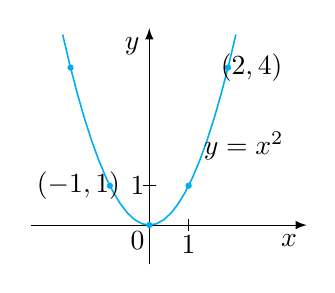
\begin{tikzpicture}
    \node at (-0.15,-0.2) {0};
    \draw[->] (-1.5,0) -- (2,0) node[below left] {$x$};
    \draw[->] (0,-0.5) -- (0,2.5) node[below left] {$y$};
    
    \draw[blueline,domain=-2.2:2.2] plot (\x/2,{(\x)^2/2});
    \foreach \x in {1,...,5}{
      \fill[bookblue] ({(\x-3)/2},{(\x-3)^2/2}) circle (0.4mm);
      %\fill[bookpink] ({\st*(\qtd - \qtd/\x)},0) circle (0.6mm);
    }
    \node at (0.5,-0.25) {$1$};
    \node at (-0.15,0.5) {$1$};
    \draw (0.5,-0.08) -- (0.5,0.08);
    \draw (-0.08,0.5) -- (0.08,0.5);
    \node at (1.3,2) {$(2,4)$};
    \node at (1.2,1) {$y=x^2$};
    \node at (-0.9,0.5) {$(-1,1)$};
  \end{tikzpicture}
\end{document}